\section{Introdução}

\subsection{Problema da Queda Livre}

\begin{figure}[htb]
 \centering
 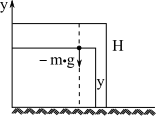
\includegraphics[scale=1.0]{capitulos/capitulo6/figuras/intro1.png}
 \caption{Problema de queda livre}
 \label{fig:intro1}
\end{figure}

Segunda Lei de Newton

\begin{equation}
 \label{cap6:sec1:eq1}
 -m \, g = m \, \frac{d^2y}{dt^2} \Rightarrow \frac{d^2y}{dt^2} = -g
\end{equation}

Chamando-se $ v = \displaystyle \frac{dy}{dt} $ reescrevemos \ref{cap6:sec1:eq1} como

\begin{equation}
 \label{cap6:sec1:eq2}
 \frac{dv}{dt} = -g
\end{equation}

Integrando-se \ref{cap6:sec1:eq2}, obtemos

\begin{equation}
 \label{cap6:sec1:eq3}
 v = -\int g \, dt = -g \, t + c_1 \Rightarrow v = -g \, t + c_1
\end{equation}

Assim

\begin{equation}
 \label{cap6:sec1:eq4}
 \frac{dy}{dt} = -g \, t + c_1
\end{equation}

Integrando-se \ref{cap6:sec1:eq4}, obtemos

\begin{equation}
 \label{cap6:sec1:eq5}
 y \, (t) = -\frac{1}{2} \, g \, t^2 + c_1 \, t + c_2
\end{equation}

Para determinarmos $ c_1 $ e $ c_2 $, precisamos de duas condições iniciais. Em

\begin{equation}
 \label{cap6:sec1:eq6}
 t = 0 \Rightarrow
 \left\{
 \begin{array}{l}
  v = v_0 \hspace*{1cm} (a)\\
  y = y_0 \hspace*{1cm} (b)
 \end{array}
 \right.
\end{equation}

De \ref{cap6:sec1:eq6}.a e \ref{cap6:sec1:eq3} temos

\begin{equation}
 \label{cap6:sec1:eq7}
 v_0 = -g \, 0 + c_1 \Rightarrow c_1 = v_0
\end{equation}

De \ref{cap6:sec1:eq7}, \ref{cap6:sec1:eq6}.b e \ref{cap6:sec1:eq5} temos

\begin{equation}
 \label{cap6:sec1:eq8}
 y_0 = -\frac{1}{2} \, g \, 0^2 + v_0 \, 0 + c_2 \Rightarrow c_2 = y_0
\end{equation}

Assim, substituindo-se \ref{cap6:sec1:eq7} e \ref{cap6:sec1:eq8} em \ref{cap6:sec1:eq5}, temos

\begin{equation}
 \label{cap6:sec1:eq9}
 y \, (t) = y_0 + v_0 \, t - \frac{1}{2} \, g \, t^2
\end{equation}

\begin{equation}
 \label{cap6:sec1:eq10}
 v \, (t) = v_0 - g \, t
\end{equation}

Suponha que o corpo é solto da altura $ H $, isto é, as condições iniciais do problema são

\begin{equation}
 \label{cap6:sec1:eq11}
 \begin{array}{lr}
  v_0 = 0 & \hspace*{1cm} (a) \\
  y_0 = H & \hspace*{1cm} (b)
 \end{array}
\end{equation}

Assim a solução do problema $ \displaystyle \frac{d^2y}{dt^2} = -g $ é

\begin{equation}
\label{cap6:sec1:eq12}
 \begin{array}{lr}
  y \, (t) = H - \displaystyle \frac{1}{2} \, g \, t^2 & \hspace*{1cm} (a) \\
  v \, (t) = -g \, t & \hspace*{1cm} (b)
 \end{array}
\end{equation}

\subsection{Problema da Queda Livre com Resistência do Ar}

\begin{figure}[htb]
 \centering
 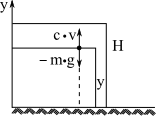
\includegraphics[scale=1.0]{capitulos/capitulo6/figuras/intro2.png}
 \caption{Problema de queda livre com resistência do ar}
 \label{fig:intro2}
\end{figure}

Segunda Lei de Newton

\begin{equation}
 \label{cap6:sec1:eq13}
 c \, v - m \, g = m \, \frac{d^2y}{dt^2}
\end{equation}

\begin{equation}
 \label{cap6:sec1:eq14}
 \frac{d^2y}{dt^2} - \frac{c}{m} \, \frac{dy}{dt} + g = 0
\end{equation}

ou

\begin{equation}
 \label{cap6:sec1:eq15}
 \frac{dv}{dt} - \frac{c}{m} \, v + g = 0
\end{equation}

ou

\begin{equation}
 \label{cap6:sec1:eq16}
 \left\{
  \begin{array}{l}
   \displaystyle \frac{dv}{dt} = f \, (v, t) \\
   \mbox{com } \, v \, (0) = v_0
  \end{array}
 \right.
\end{equation}

Estudaremos problemas do tipo \ref{cap6:sec1:eq16} onde $ \, f \, (v, t) \, $ pode, inclusive, ser uma função não-linear de $ \, v \, $.

Como resolver o problema \ref{cap6:sec1:eq15} ?

\textbf{Método analítico}

\begin{equation}
 \left\{
  \begin{array}{lr}
   \label{cap6:sec1:eq17}
   v' - a \, v = b & \hspace*{1cm} (a) \\
   %\label{cap6:sec1:eq18}
   v \, (0) = v_0 & \hspace*{1cm} (b)
  \end{array}
 \right.
\end{equation}

Multiplicando-se \ref{cap6:sec1:eq17}.a por $ \, e^{-a\,t} \, $ temos

\begin{equation}
 \label{cap6:sec1:eq19}
 e^{-a\,t} \, (v' - a \, v) = e^{-a\,t} \, b
\end{equation}

Mas

\begin{equation}
 \label{cap6:sec1:eq20}
 \frac{d}{dt} \, (v \, e^{-a\,t}) = v' \, e^{-a\,t} - a \, v \, e^{-a\,t} = e^{-a\,t} \, (v' - a \, v)
\end{equation}

Assim \ref{cap6:sec1:eq19} fica

\begin{equation}
 \label{cap6:sec1:eq21}
 \frac{d}{dt} \, (v \, e^{-a\,t}) = e^{-a\,t} \, b
\end{equation}

Integrando-se \ref{cap6:sec1:eq21}, temos

\begin{equation}
 \label{cap6:sec1:eq22}
 e^{-a\,t} = - \frac{b}{a} \, e^{-a\,t} + c_1
\end{equation}

Aplicando-se a condição inicial \ref{cap6:sec1:eq17}.b a \ref{cap6:sec1:eq22}, temos

\begin{equation}
 \label{cap6:sec1:eq23}
 ? e^0 \, v_0 = - \frac{b}{a} \, e^0 + c_1 - c_1 = v_0 + \frac{b}{a} ?
\end{equation}

Substituindo-se \ref{cap6:sec1:eq23} em \ref{cap6:sec1:eq22} e multiplicando-se por $ \, e^{-a\,t} \, $, temos

\begin{equation}
 \label{cap6:sec1:eq23}
 \mbox{ \framebox{ $ v \, (t) = v_0 \, e^{a\,t} + \displaystyle \frac{b}{a} \, (e^{a\,t} - 1) $ } }
\end{equation}

OBS: Exemplos de equações diferenciais ordinárias:

\[
 \begin{array}{l}
  1^{_a} \mbox{ ordem: } v' - a \, v = f \, (t) \\
  2^{_a} \mbox{ ordem: } v'' + p \, v + q \, v = f \, (t)
 \end{array}
\]

\begin{example}
 Resolveremos o problema de valor inicial dado nas equação abaixo de forma exata, usando a técnica mostrada em sala de aula para as seguintes condições iniciais: y{}_{0}=2000m e v_{0}=-2m/s . Considere g=10m/s^{2} , M = 50 kg e o coeficiente de empuxo k = 50 N * s /m .

Dados:

\begin{cases}
M*\frac{d^{2}y(t)}{dt^{2}}=-M*g-k*v(t) & (1)\\
y(0)=y_{0} & (2)\\
\frac{dy}{dt}(0)=v_{0} & (3)\end{cases}

Temos que:

\frac{d^{2}y(t)}{dt^{2}}=\frac{dv(t)}{dt}(4)

Substituindo (4) em (1):

M*\frac{dv(t)}{dt}=-M*g-k*v(t)

Desenvolvendo:

\frac{dv(t)}{dt}=-g-\frac{k}{M}*v(t)

\begin{cases}
\frac{dv}{dt}=f(v,t)\\
v(0)=v_{0}\end{cases}

Usando o artifício mostrado na demonstração 6.18 da apostila, teremos:

a=\frac{k}{M}

e^{at}(v'+av)=-ge^{at}

e^{at}*\frac{dv(t)}{dt}=-g*e^{at}-a*v(t)*e^{at}

Integrando:

\int d(e^{at}*v(t))=-g\int e^{at}dt

Teremos:

e^{at}v(t)=-g*\frac{e^{at}}{a}+c1

v(t)=(\frac{-g}{a})+\frac{c1}{e^{at}}

Com \frac{dy}{dt}(0)=v_{0}=v(0), temos para t=0:

v(0)=(\frac{-g}{a})+\frac{c1}{e^{a*0}}

c1=v_{0}+\frac{g}{a}

Então:

v(t)=(\frac{-g}{a})+\frac{v_{0}+\frac{g}{a}}{e^{at}}

Desenvolvendo 3 em funcao de t:

\frac{dy}{dt}(t)=v(t)

dy(t)=v(t)dt

Integrando os 2 lados:

\int dy(t)=\int v(t)dt

y(t)=\int(\frac{-g}{a})dt+\int\frac{v_{0}+\frac{g}{a}}{e^{at}}dt

y(t)=(\frac{-g}{a})t+(v_{0}+\frac{g}{a})*\int e^{-at}dt

y(t)=(\frac{-g}{a})t+(v_{0}+\frac{g}{a})*\frac{e^{-at}}{-a}+c2

Para y(0)=y{}_{0}, temos:

y(0)=0+(v_{0}+\frac{g}{a})*\frac{1}{-a}+c2

c2=y_{0}+(v_{0}+\frac{g}{a})*\frac{1}{a}

Então,

y(t)=(\frac{-g}{a})t+(v_{0}+\frac{g}{a})*\frac{e^{-at}}{-a}+y_{0}+(v_{0}+\frac{g}{a})*\frac{1}{a}

y(t)=(\frac{-g}{a})t+y_{0}+(v_{0}+\frac{g}{a})*(\frac{1}{a})*(1-e^{-at})

Usando os valores dados como condições iniciais: y{}_{0}=2000m e v_{0}=-2m/s . Considere g=10m/s^{2} , M = 50 kg e o coeficiente de empuxo k = 50 N ⋅ s /m, teremos:

a=\frac{k}{M}=1

Velocidade:

v(t)=(\frac{-g}{a})+\frac{v_{0}+\frac{g}{a}}{e^{at}}=(\frac{-10}{1})+\frac{(-2)+\frac{10}{1}}{e^{1t}}

v(t)=-10+\frac{8}{e^{t}}

Espaço:

y(t)=(\frac{-g}{a})t+y_{0}+(v_{0}+\frac{g}{a})*(\frac{1}{a})*(1-e^{-at})

y(t)=(\frac{-10}{1})t+2000+(-2+\frac{10}{1})*(\frac{1}{1})*(1-e^{-1t})

y(t)=-10t+2008+-8*e^{-t})
\end{example}


\subsection{Métodos Numéricos para Problemas de Valor-Inicial}

A solução exata do problema

\[
 \left\{
  \begin{array}{ll}
   u' = f \, (t, u) & \hspace*{1cm} \mbox{E.D.O} \\
   u \, (0) = u_0 & \hspace*{1cm} \mbox{I.C.}
  \end{array}
 \right.
\]

É contínua no tempo. Nos métodos numéricos tentamos acompanhar a solução de forma discreta do tempo. Assim, começando de $ \, u \, (0) = u_0 \, $, damos um passo finito $ \, \Delta t \, $ de cada vez e esperamos que depois de $ \, n \, $ passos a solução numérica $ \, u_n \approx u \, (n \, \Delta t) \, $.

Devemos nos preocupar com:

\begin{enumerate}

\item \textbf{Precisão}: o erro $ \, u \, (n \, \Delta t) - u_n \, $ tem a seguinte forma $ \, E = C \, (\Delta t)^p \, $. Para reduzir o erro podemos aumentar a ordem de precisão, $ \, p \, $, ou diminuir $ \, \Delta t \, $.

\item \textbf{Simplicidade}: o passo de $ \, u_n \, $ para $ \, u_{n+1} \, $ pode ser rápido ou vagaroso, dependendo da quantidade de vezes que calculamos $ \, f \, (t, u) \, $.

\item \textbf{Estabilidade}: em cada passo, pequenos erros são introduzidos. Se o erro acumulado crescer de forma descontrolada o resultado é inútil.

\end{enumerate}

Procedimento numérico (método da variável discreta): constrói valores aproximados

\[
 u_0, \, u_1, \, u_2, \, \ldots \, , \, u_n, \, \ldots
\]

da solução exata nos tempos

\[
 t_0, \, t_1, \, t_2, \, \ldots \, , \, t_n, \, \ldots
\]

dada por

\[
 u \, (t_0), \, u \, (t_1), \, u \, (t_2), \, \ldots \, , \, u \, (t_n), \, \ldots
\]

Como determinar $ \, u_1 \, $ a partir de $ \, u_0 \, $ e $ \, f \, (t_0, u_0) \, $ ?\\

\textbf{Métodos}

\begin{itemize}

\item \textit{One-step} (passo-simples)

\item \textit{Stepwise} (passo-a-passo)

\item \textit{Starting methods} (de inicialização)

\end{itemize}

Precisam do conhecimento de $ \, u_n \, $ para determinar $ \, u_{n+1} \, $.\\

\textbf{Métodos}

\begin{itemize}

\item \textit{Multistep} (passo-múltiplo)

\item \textit{Continuing Methods} (de continuação)

\end{itemize}

Precisam do conhecimento de $ \, u_n, \, u_{n-1}, \, \ldots \, $ para determinar $ \, u_{n+1} \, $\\

OBS: Todo método de passo-múltiplo precisa de um método de inicialização (passo-simples) para obter os valores iniciais do método.\\

Qual a sensibilidade da solução com relação às condições iniciais ou a outros parâmetros do problema?\\

Convergência: $ \, \Delta t \rightarrow 0 \Rightarrow y_i \rightarrow u \, (t_i) \, $ ?

Erros:

\begin{itemize}

\item Fórmula (ou truncamento, ou discretização)

\item Erro de arredondamento

\end{itemize}
